\chapter{Web interface}
\label{chap:web-interface}
\index{sg-web}

  The command-line programs described in chapter \refer{chap:command-line}
  provide data for layer \t{0}.  With the web interface described in
  this chapter, this data can be further structured, analyzed, and shared.
  In short, with the web interface you can:
  \begin{itemize}
  \item Manage data and data access across RDF stores;
  \item Write, execute, and share SPARQL queries;
  \item Explore the inner-structure of datasets.
  \end{itemize}

\section{Setting up the web interface}
\label{sec:configuring-sg-web}

  Before the web interface can be started, a few parameters have to be
  configured.  This is done through an XML file.  The following example
  displays all options, except for the authentication part, which is
  discussed separately in section \refer{sec:authentication}.

\begin{siderules}
\begin{verbatim}
<?xml version="1.0" encoding="utf-8"?>
<web-interface>
  <fork>0</fork>
  <bind-address>127.0.0.1</bind-address>
  <port>8080</port>
  <developer-mode>0</developer-mode>
  <backtrace-on-error>0</backstrace-on-error>
  <system-connection>
    <uri>http://localhost:8890/sparql-auth</uri>
    <backend>virtuoso</backend>
    <username>dba</username>
    <password>dba</password>
  </system-connection>
  <authentication>
    <!-- Either LDAP settings, or local-user authentication -->
  </authentication>
</web-interface>
\end{verbatim}
\end{siderules}

\subsection{To fork or not to fork}

  The \t{fork} property can be either \t{0} to keep the
  \program{sg-web} process in the foreground of your shell, or
  \t{1} to run the \program{sg-web} process as a daemon.

\subsection{Bind address and port}

  To enable running multiple web services on single machine, \program{sg-web}
  can be configured to bind on an arbitrary address and an arbitrary port.
  Both IPv4 and IPv6 addresses are supported.

\subsection{Developer mode}

  By default, changes to code in the \file{www/pages/} directory are
  applied when restarting \program{sg-web}.  When turning on
  `\t{developer-mode}', pages are reloaded when accessed, which makes
  interactive development of web pages easier.

\subsection{Logging and backtraces}
\label{sec:logging}

  The \program{sg-web} program keeps two logs: one for error reporting, and
  one for access and non-critical messages.  The log files can be specified
  as command-line options (\t{-e} for error reporting, \t{-d} for
  non-critical messages).

  Backtraces help the developer to get an idea about how something might've
  gone wrong.  It displays the location nearby the location in the source code
  that throwed an error.  Backstraces can get long and verbose.  Therefore we
  don't display them by default.  To enable reporting backtraces in the error
  log, set the `\t{backtrace-on-error}' option to \t{1}.

\subsection{System connection}

  The web interface stores its own information as RDF.  Therefore it needs
  a connection to an RDF store where it can write to the graphs described
  in table \ref{table:writable-graphs}.

  \hypersetup{urlcolor=black}
  \begin{table}[H]
    \begin{tabularx}{\textwidth}{l!{\VRule[-1pt]}X}
      \headrow
      \b{Graph} & \b{Reason}\\
      \evenrow
      \t{http://sparqling-genomics.org/sg-web/state}
      & In this graph, queries and projects are stored.\\
    \end{tabularx}
    \caption{\small Graphs that need to be writable for the web interface.}
    \label{table:writable-graphs}
  \end{table}
  \hypersetup{urlcolor=LinkGray}

\subsubsection{System connection example}

  To configure the \i{system connection}, two parameters need to be
  specified: \t{uri}, and \t{backend}.  Additionally, when the
  RDF store requires authentication for writing to it, a \t{username}
  and a \t{password} can be provided.

  The following example shows how to configure the \i{system connection}:

\begin{siderules}
\begin{verbatim}
<?xml version="1.0" encoding="utf-8"?>
<web-interface>
  ...
  <system-connection>
    <uri>http://localhost:8890/sparql-auth</uri>
    <backend>virtuoso</backend>
    <username>dba</username>
    <password>dba</password>
  </system-connection>
</web-interface>
\end{verbatim}
\end{siderules}

\subsection{Beacon support}
\label{sec:beacon}

  Beacon is an interface to create a ``global search engine for genetic
  mutations'' \citep{beacon-network}.  It achieves this by defining a
  standard that institutions must implement so that one search engine can
  query the implementations from each institution to find a specific
  genetic mutation.

  The web interface can function as a Beacon in the Beacon network
  \citep{beacon-network}.  The Beacon API uses a separate connection,
  similar to the \t{system-connection}, so that access can be
  controlled at the user level.

  The following example shows how to configure \i{Beacon} including the
  \i{Beacon connection}:

\begin{siderules}
\begin{verbatim}
<?xml version="1.0" encoding="utf-8"?>
<web-interface>
  ...
  <beacon>
    <enabled>1</enabled>
    <organization>
      <id>SG</id>
      <name>SPARQLing-genomics Beacon service</name>
      <description>
        This Beacon service provides variant information for data hosted by
        this instance of the RDF store.
      </description>
      <address>Not provided</address>
      <welcome-url>https://www.sparqling-genomics.org</welcome-url>
      <contact-url>mailto:beacon@sparqling-genomics.org</contact-url>
      <logo-url>https://www.sparqling-genomics.org/static/images/logo.png</logo-url>
      <info>Not provided</info>
    </organization>
    <connection>
      <uri>http://localhost:8000</uri>
      <backend>virtuoso</backend>
      <username>beacon</username>
      <password>changeme</password>
    </connection>
  </beacon>
</web-interface>
\end{verbatim}
\end{siderules}

  The implementation assumes the following conditions are met:
  \begin{itemize}
  \item Variant call data was imported using \t{vcf2rdf};
  \item The reference genome can be identified by the chromosome's NCBI
    identifier.
  \end{itemize}

\subsection{User management and authentication}
\label{sec:authentication}

  The \program{sg-web} assumes every user of the system has a username
  and a password to authenticate oneself. There are three ways to configure
  authentication.  For isolated deployments or environments, preconfigured
  accounts can be specified.  For organizational deployments, the web interface
  can be configured to use an LDAP server that supports version 3 of the LDAP
  protocol.  For public access deployments, ``log in with ORCID'' can be
  configured.

  Regardless of the authentication mechanism, there are a few reserved users
  that carry out a specific task within \program{sg-web}.  The table below
  describes the reserved users.

  \hypersetup{urlcolor=black}
  \begin{table}[H]
    \begin{tabularx}{\textwidth}{l!{\VRule[-1pt]}X}
      \headrow
      \b{Username} & \b{Task}\\
      \evenrow
      \t{beacon}
      & When the BEACON API (see section \refer{sec:beacon}) is enabled, and
      this user is added to a project, the data that is accessible by the
      project will be exposed to the BEACON network.\\
      \oddrow
      \t{portal}
      & This username has been reserved for an implementation of a data
      portal.\\
    \end{tabularx}
    \caption{\small Reserved users for \program{sg-web}.}
    \label{table:reserved-users}
  \end{table}
  \hypersetup{urlcolor=LinkGray}

\subsubsection{Local users configuration}

  The simplest form of authentication is the ``local-user configuration''.
  Configuring it involves providing a username and the SHA256 sum of a password
  for each account.  The following example shows how to configure
  ``local-user authentication'':

\begin{siderules}
\begin{verbatim}
<?xml version="1.0" encoding="utf-8"?>
<web-interface>
  ...
  <authentication>
    <user>
      <username>user</username>
      <!-- The password field must contain the SHA256 sum of the
           plaintext password -->
      <password>9f86d08...0f00a08</password>
    </user>
    <user>
      <username>user2</username>
      <password>152f347...0b7a26a</password>
    </user>
  </authentication>
</web-interface>
\end{verbatim}
\end{siderules}

\subsubsection{LDAP authentication example}

  To configure LDAP, four parameters must be specified: the URI to the LDAP
  service (1), optionally, an extra ``common name'' (2), optionally the
  ``organizational unit'' (3), and the ``domain'' (4).  The username is used
  as a ``common name''.

  \begin{sloppypar}
  Additionally, an alternative SSL certificate bundle can be configured with
  the parameters \t{ssl-certificate-directory} and
  \t{ssl-certificate-file}.
  \end{sloppypar}

  The following example shows how to configure LDAP authentication:

\begin{siderules}
\begin{verbatim}
<?xml version="1.0" encoding="utf-8"?>
<web-interface>
  ...
  <authentication>
    <ldap>
      <uri>ldaps://example.local</uri>
      <common-name>AdditionalCN</common-name>
      <organizational-unit>People</organizational-unit>
      <domain>department.organization.tld</domain>
      <ssl-certificate-directory>/etc/ssl/certs</ssl-certificate-directory>
      <ssl-ca-certificate-file>
        /etc/ssl/certs/ca-certificates.crt
      </ssl-ca-certificate-file>
    </ldap>
  </authentication>
</web-interface>
\end{verbatim}
\end{siderules}

\subsubsection{ORCID authentication example}

  To configure ``login with ORCID'', four parameters must be specified:
  the \t{client-id} (1) and \t{client-secret} (2) which are provided
  when registering your application at ORCID.  The \t{endpoint} (3) which
  should always be \t{https://orcid.org/oauth}, and the \t{redirect-uri}
  (4) that is used to redirect to when a user has logged into ORCID and
  authorized the login request.  The default path to redirect to should
  be \t{/login}.  Internally, the ORCID ID is used as identifier for a user.

  The following example shows how to configure ORCID authentication:

\begin{siderules}
\begin{verbatim}
<?xml version="1.0" encoding="utf-8"?>
<web-interface>
  ...
  <authentication>
    <orcid>
      <client-id>APP-XXXXXXXXXXXXXXXX</client-id>
      <client-secret>XXXXXXXX-XXXX-XXXX-XXXX-XXXXXXXXXXXX</client-secret>
      <endpoint>https://orcid.org/oauth</endpoint>
      <redirect-uri>https://<your-public-uri>/login</redirect-uri>
    </orcid>
  </authentication>
</web-interface>
\end{verbatim}
\end{siderules}

\subsection{Running the web interface}

  The web interface can be started using the \program{sg-web} command:

\begin{siderules}
\begin{verbatim}
sg-web --configuration-file=file.xml
\end{verbatim}
\end{siderules}

  $\ldots{}$ where \t{file.xml} is a configuration file as
  discussed in section \refer{sec:configuring-sg-web}.

\pagebreak{}
\section{Managing multi-node setups with \program{sg-auth-manager}}

  When the knowledge graph grows beyond the capabilities of a single machine,
  one can consider scaling out to another.  The provided solution to manage
  multiple RDF stores while maintaining a single-point-of-entry for users
  involves running helper program called \program{sg-auth-manager} alongside
  a secondary RDF store.  This program communicates with \program{sg-web} to
  manage permissions, and handle data import and export.  Figure
  \ref{fig:sg-auth-manager} provides a schematic overview of the deployment
  model.

  \begin{figure}[H]
    \begin{center}
    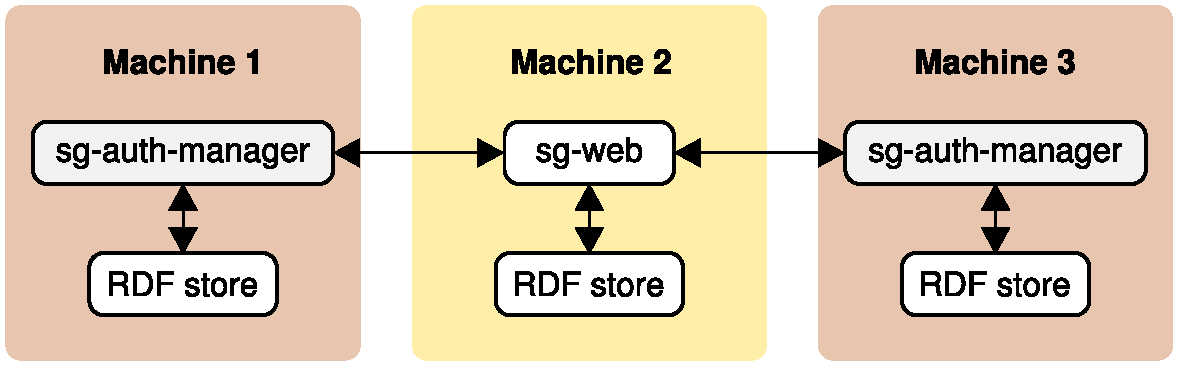
\includegraphics[width=0.8\textwidth]{figures/sg-auth-manager-scaleout.pdf}
    \end{center}
    \caption{\textit{Illustrating a three-node setup.}}
    \label{fig:sg-auth-manager}
  \end{figure}

  %At least one instance of \program{sg-web} must run, so that the
  %\program{sg-auth-manager} can verify the validity of a request that was sent
  %to it.

  The \program{sg-auth-manager} program verifies the validity of the user's session
  token with the \program{sg-web} instance before acting as a proxy to the managed
  RDF store.

\subsection{Importing data into secondary stores}

  RDF importing is handled by an API call to the instance managed by
  \program{sg-auth-manager}.

  When \program{sg-web} receives a request to import data into an
  \program{sg-auth-manager}-managed RDF store, it passes the data directly
  to the \program{sg-auth-manager}, which in turn handles the importing of data
  into that store.

\subsection{How \program{sg-web} handles downtime of a \program{sg-auth-manager}}

  The \program{sg-auth-manager} registers itself with the pre-configured
  \program{sg-web} instance upon start.  In turn, the \program{sg-web} instance
  polls the availability of the \program{sg-auth-manager} instance every 10
  seconds.  When the \program{sg-auth-manager} instance is unavailable for 30
  consecutive seconds, \program{sg-web} removes the connection, and the
  \program{sg-auth-manager} instance must re-register itself.

\subsection{Federated querying of protected endpoints}

  The \t{sg-auth-manager} provides a mechanism to execute federated queries
  using protected endpoints by allowing the session token (see section
  \ref{sec:tokens}) as part of the URI in the \t{SERVICE} specification.

\pagebreak{}
\section{Testing a running instance of \t{sg-web}.}

  The test suite used to prevent functional regressions between releases is
  available in the \t{sg-web-test} program.  This program can be used to test
  whether all features from the API are working correctly after deployment.

  The program can perform two types of tests: \t{endpoint-test} and
  \t{sparql-parser-test}.

\subsection{Testing an endpoint}

  The \t{endpoint-test} interacts with an endpoint through its API.  To run
  this test, invoke \program{sg-web-test} as following:

\begin{siderules}
\begin{verbatim}
sg-web-test --endpoint https://www.sparqling-genomics.org --token TOKEN
\end{verbatim}
\end{siderules}

  Replace \t{https://www.sparqling-genomics.org} with your endpoint's
  address, and \t{TOKEN} with an access token for your endpoint.

\subsection{Testing the SPARQL parser}

  To detect defects in the SPARQL parser, we use the \t{sparql-parser-test}
  to parse queries from \t{*.sparql} files from a directory.  To start this
  test, invoke \program{sg-web-test} as following:

\begin{siderules}
\begin{verbatim}
sg-web-test --sparql-parser /path/to/directory/with/queries
\end{verbatim}
\end{siderules}

\pagebreak{}
\section{Using the web interface}
\label{sec:using-web-interface}

  Once the web interface is up and running, a logged-in user will land
  on the \i{Dashboard}.

  \begin{figure}[H]
    \begin{center}
      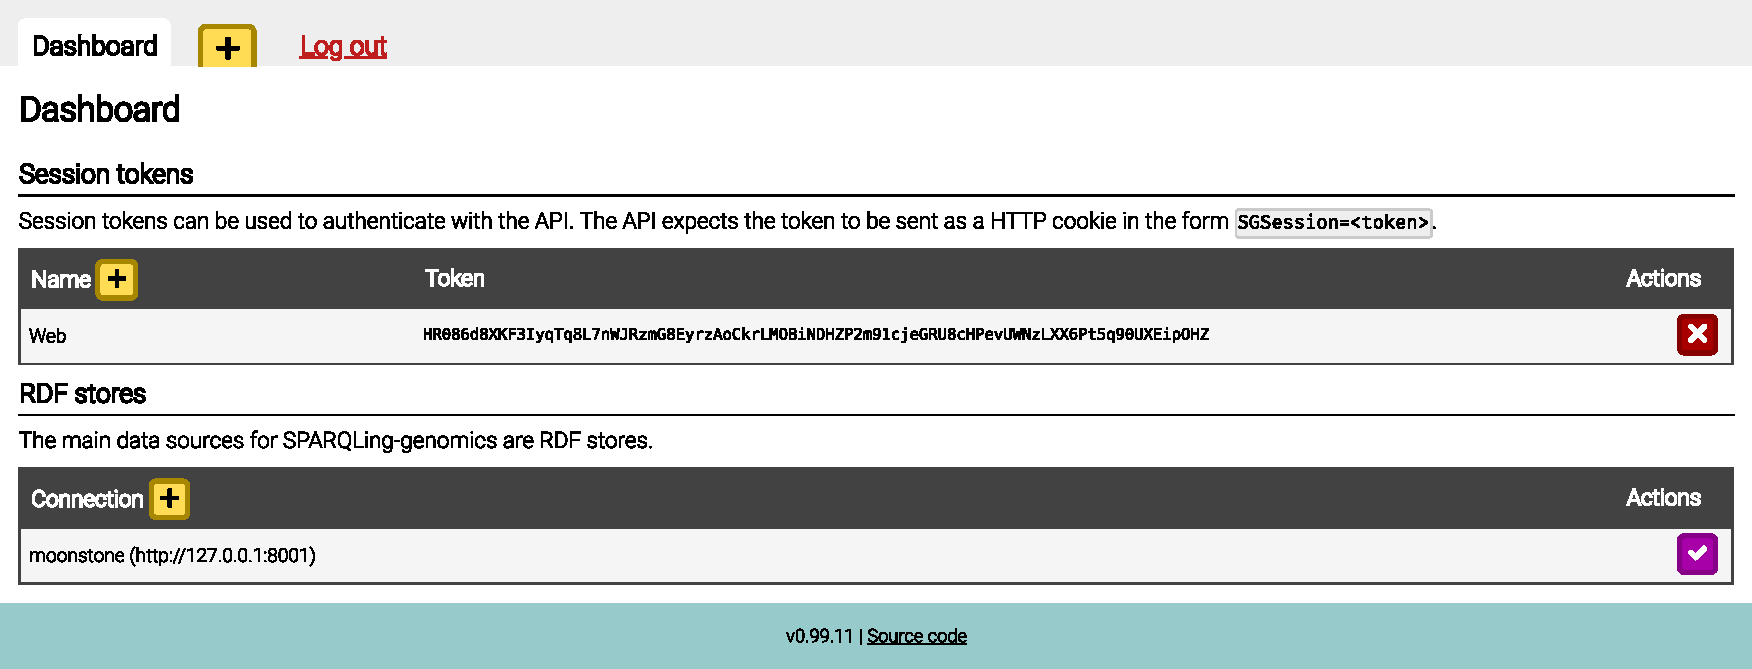
\includegraphics[width=1.0\textwidth]{figures/sg-web-dashboard.pdf}
    \end{center}
    \caption{On the \i{Dashboard}, tokens and connections can be
      configured.}
    \label{fig:web-dashboard}
  \end{figure}

  The dashboard provides access to two resources: \i{session tokens}
  and \i{RDF stores}.  Session tokens will be discussed in section
  \refer{sec:tokens}.  This leaves us with \i{RDF stores} for now.

\subsection{Configuring connections}
\label{sec:configure-connections}

  The web interface supports two types of connections; \i{user-specific
    connections} and \i{system-wide connections}.  Users can add the
  former using the \t{+} button.  Such a connection will only be visible
  to the user who added it.  On the contrary, \i{system-wide connections}
  are visible to all users.

  System-wide connections are therefore not configured by a user, but by a
  program called \program{sg-auth-manager}.  This program works as a middle-man
  between a private RDF store, and a running instance of \program{sg-web}.  It
  uses the user management from \program{sg-web} described in section
  \refer{sec:authentication} to allow users to access graphs assigned to one
  of their projects.

  An instance of \program{sg-auth-manager} registers itself with
  \program{sg-web} as a system-wide connection: making itself available to
  all users of the \program{sg-web} instance.

\subsection{Projects}
\label{sec:web-projects}

  The main way to access the knowledge graph, and to collaborate with other
  users is through a \i{project}.  Projects combine \i{users},
  \i{access to data} and \i{queries}.  The structure of a project
  attempts to capture general phases of analyzing data: \i{collect}
  $\rightarrow$ \i{structure} $\rightarrow$ \i{query} $\rightarrow$
  \i{report} $\rightarrow$ \i{automate}.

  \begin{figure}[H]
    \begin{center}
      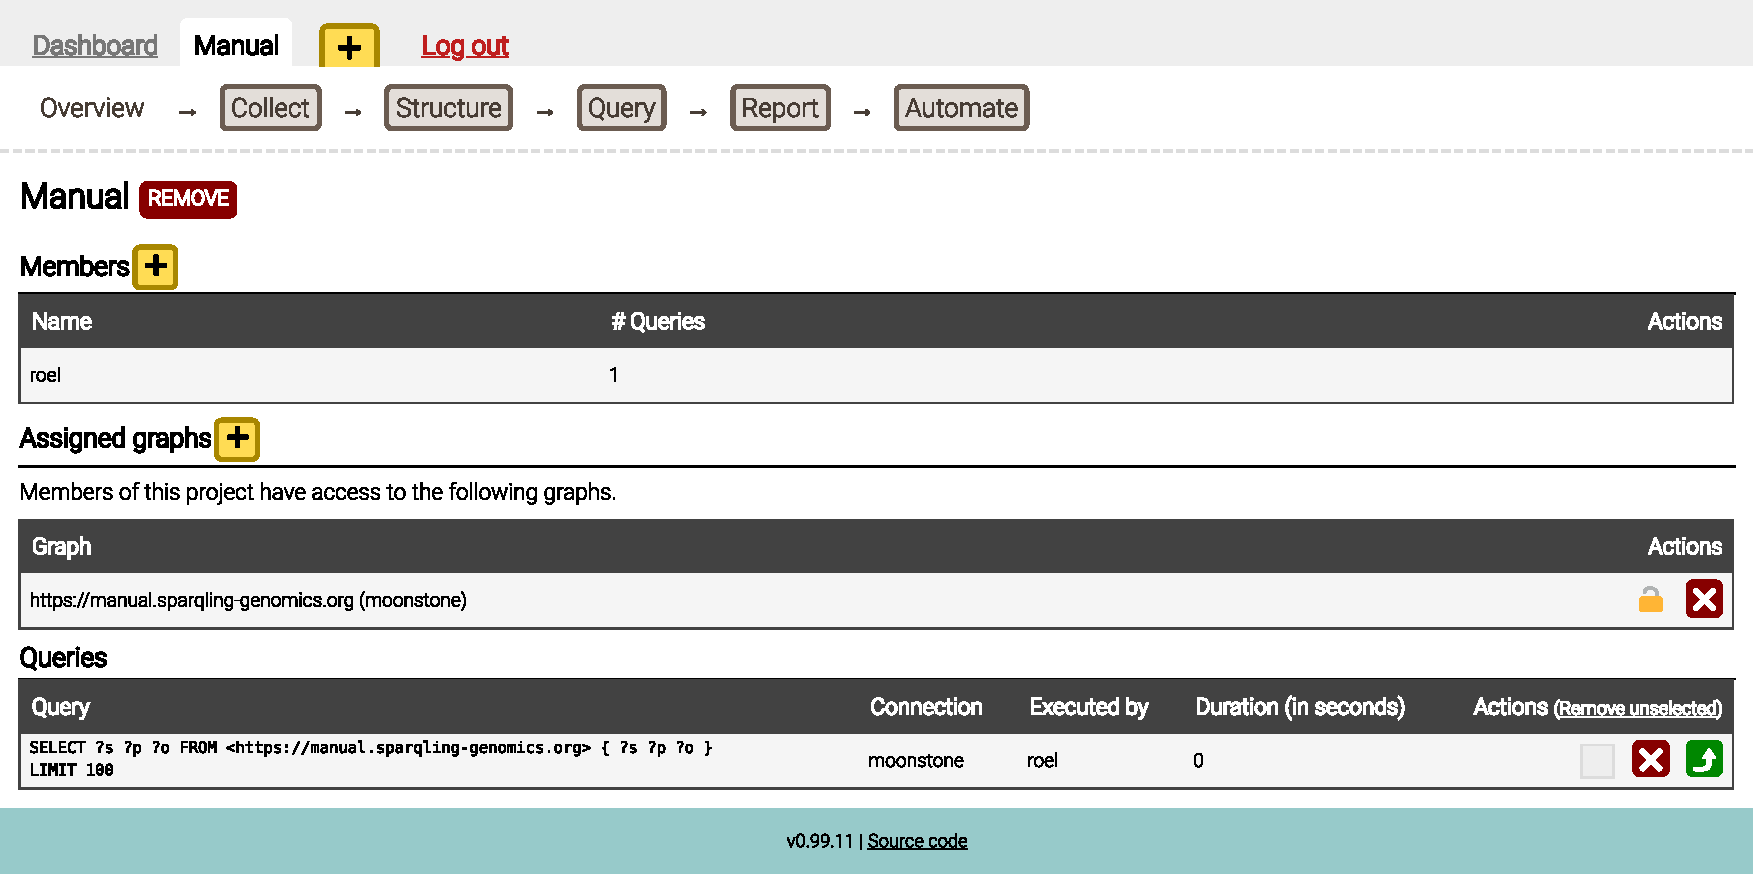
\includegraphics[width=1.0\textwidth]{figures/sg-web-project-details.pdf}
    \end{center}
    \caption{The project overview page.}
    \label{fig:web-project-overview}
  \end{figure}

\subsubsection{Collecting data}

  Before data can be analyzed, it must be collected and stored.  Graphs are
  the primary place to store data.  Graphs are identified by a uniform resource
  identifier (URI).  So before data can be imported, a project must assign a
  graph.

  After assigning a graph to the project on the \i{Overview} page, the
  command to load a file can be generated in three steps.

  \begin{figure}[H]
    \begin{center}
      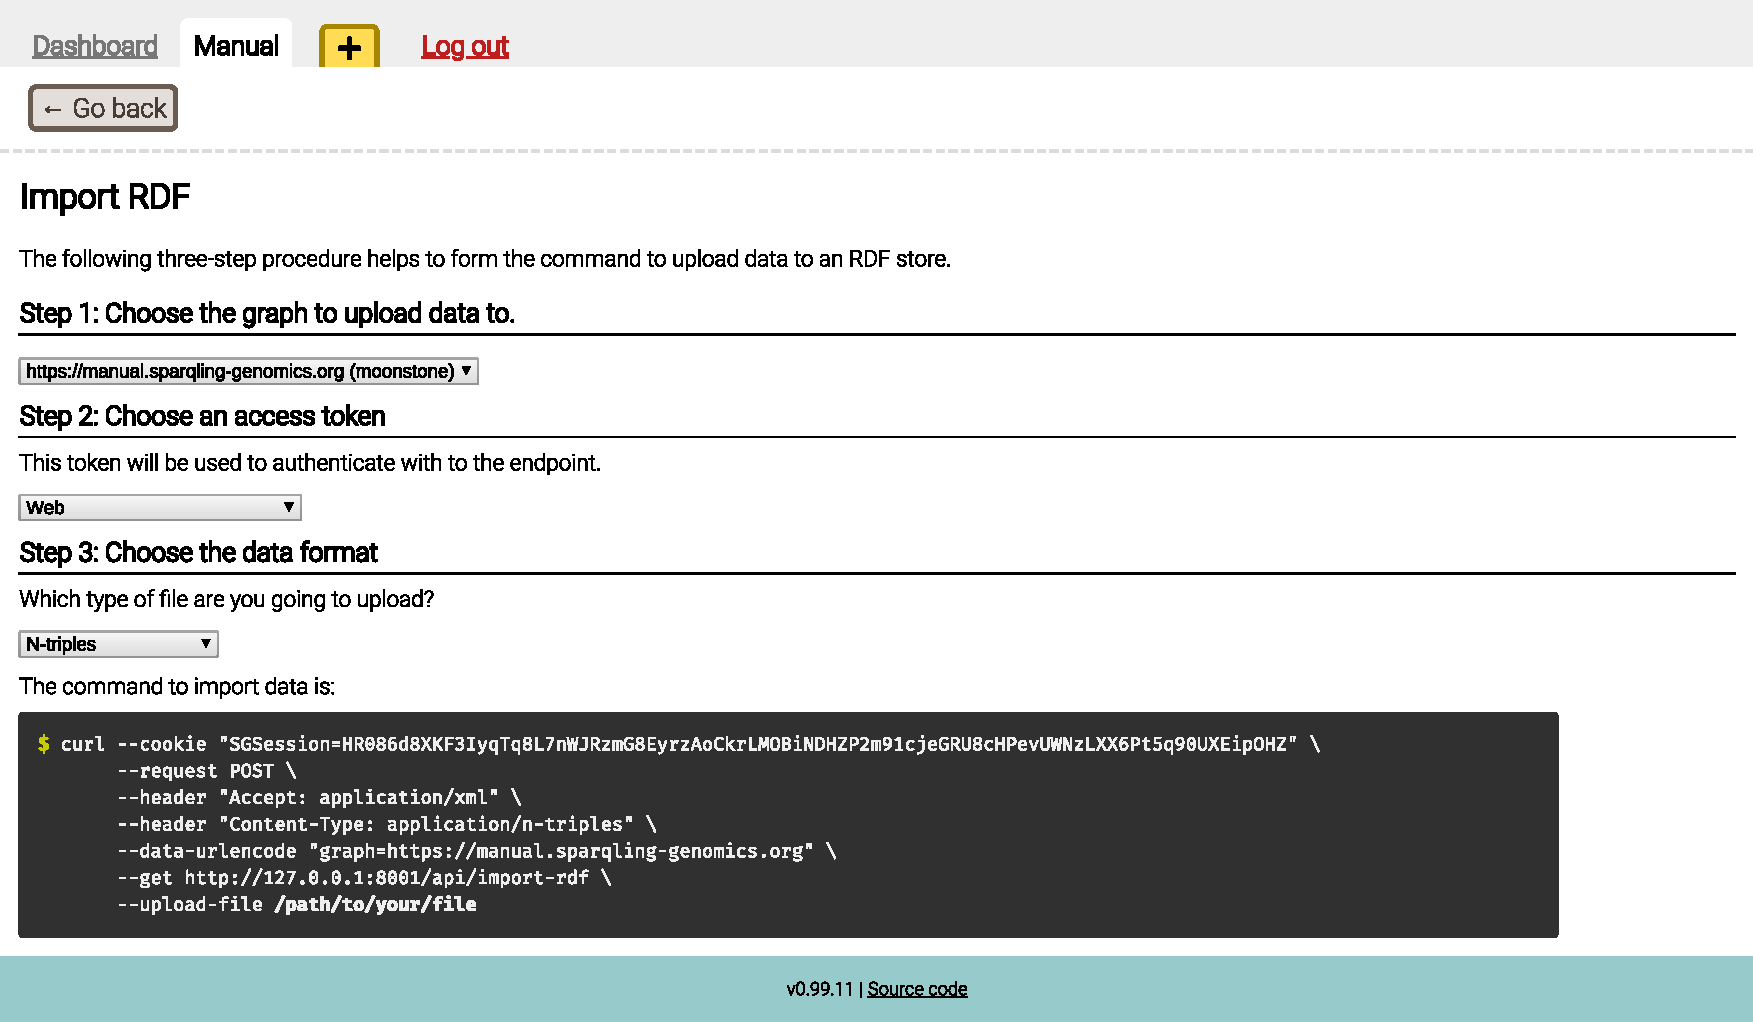
\includegraphics[width=1.0\textwidth]{figures/sg-web-import-rdf.pdf}
    \end{center}
    \caption{Importing RDF in three steps}
    \label{fig:web-import-rdf}
  \end{figure}

\subsection{Executing queries}

  After configuring at least one endpoint, it can be chosen on the \i{query}
  page to execute a query against it.

  \begin{figure}[H]
    \begin{center}
      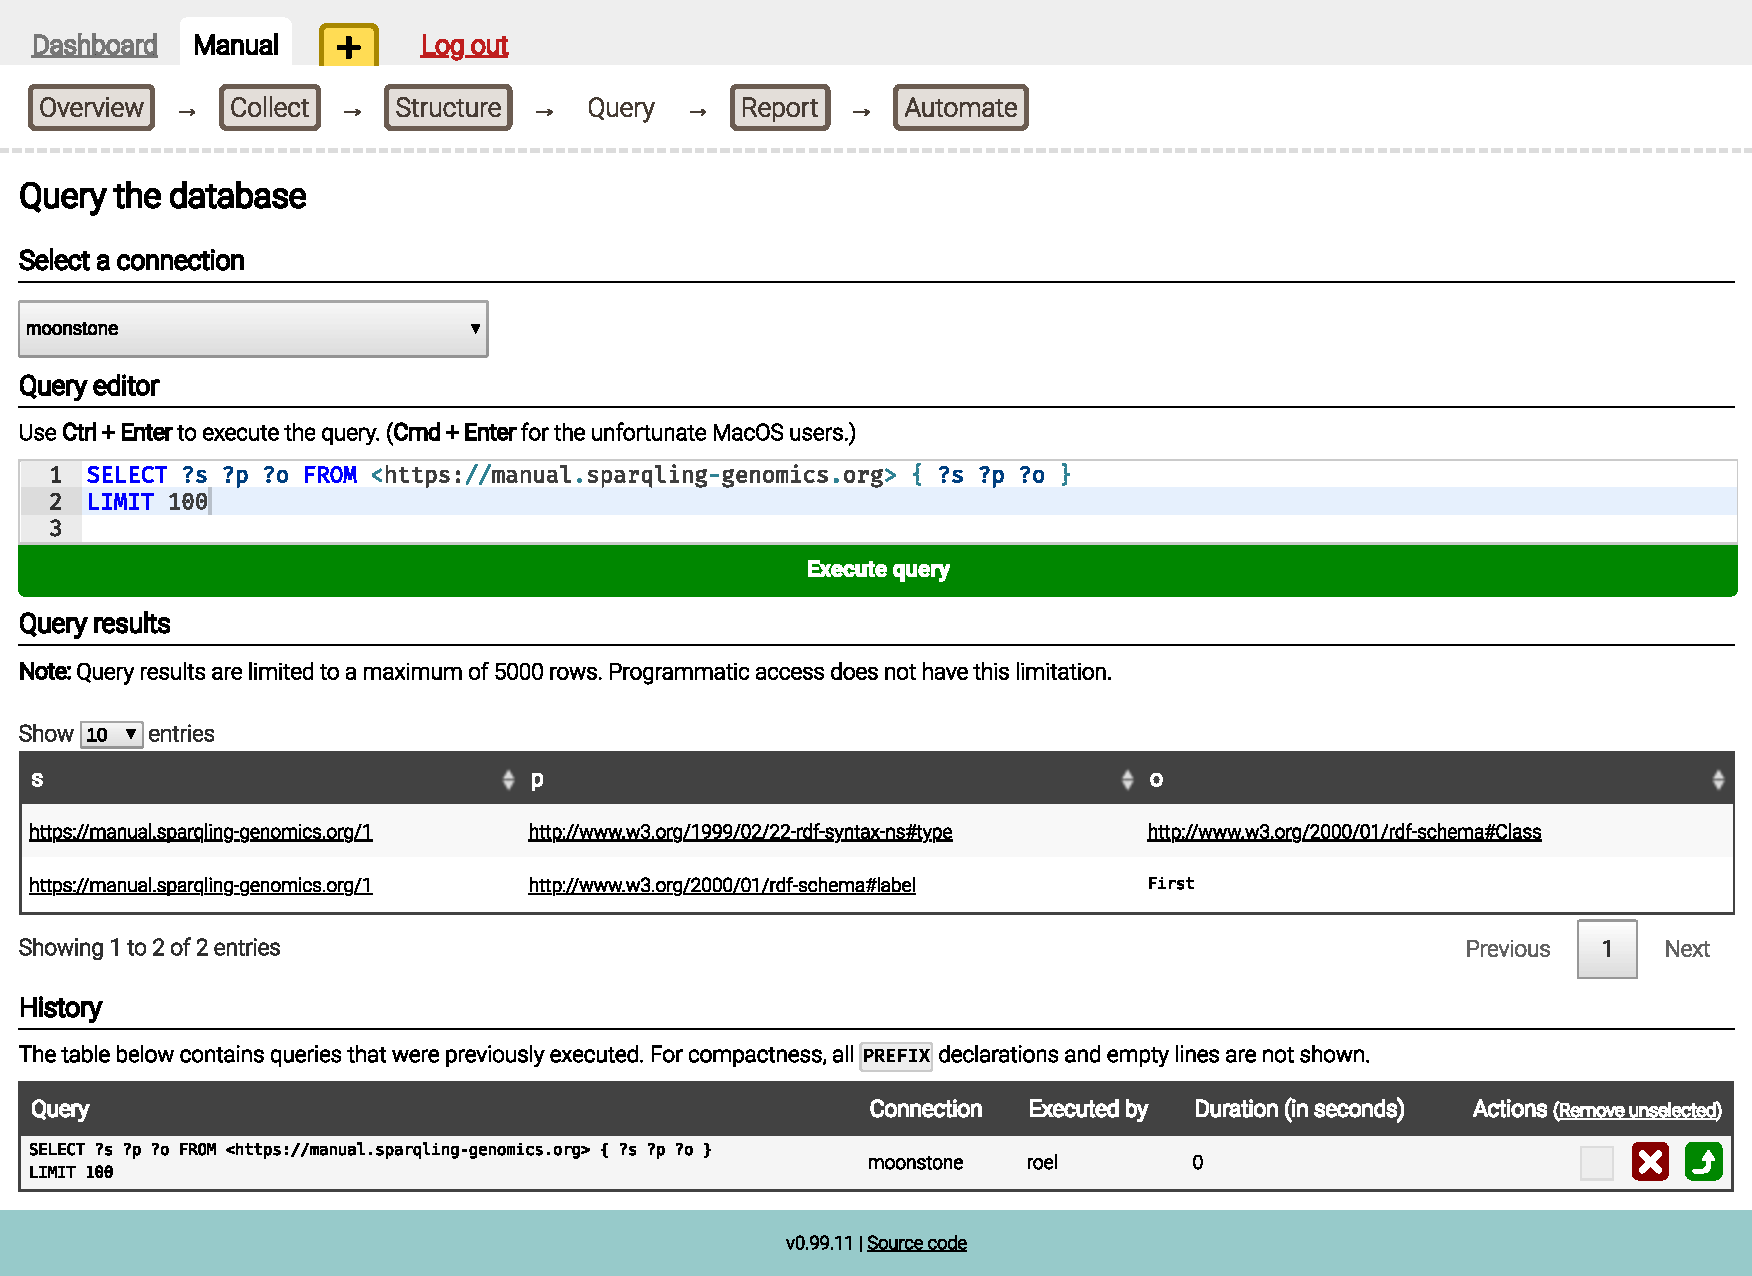
\includegraphics[width=1.0\textwidth]{figures/sg-web-query.pdf}
    \end{center}
    \caption{The \i{query} page enables users to execute a query against a
      SPARQL endpoint.  The connections configured at the \i{connections} page
      can be chosen from the drop-down menu.}
    \label{fig:web-query}
  \end{figure}

\subsection{Query history}
\label{sec:query-history}

  When prototyping SPARQL queries, better known as ``SPARQLing around'', it's
  good to know that all queries that yielded a result are stored in the
  \i{query history}.  The history is shown on the \i{query} page below the
  query editor.  Each \i{project} has its own query history.

\subsection{Explore graphs with the Exploratory}

  Another utility aimed at SPARQLing around faster is the \i{exploratory}.

  \begin{figure}[H]
    \begin{center}
      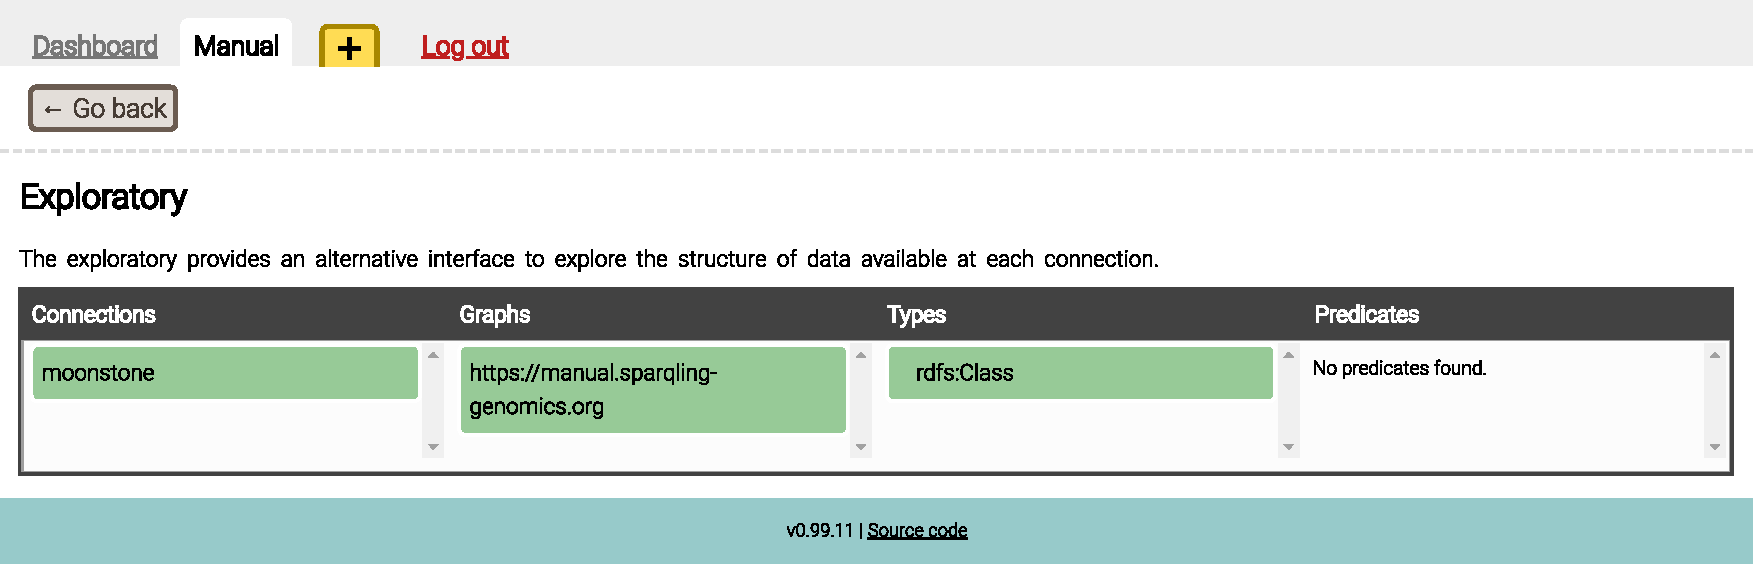
\includegraphics[width=1.0\textwidth]{figures/sg-web-exploratory.pdf}
    \end{center}
    \caption{The \i{exploratory} page enables users to learn about the
      structure of the triplets in a graph.}
    \label{fig:web-exploratory}
  \end{figure}

  The exploratory uses a common pattern in RDF to help writing queries.  Its
  interface provides a four-step selection process to find \i{predicates}
  associated with an \t{rdf:type}.  The programs described in chapter
  \refer{chap:command-line} automatically add the \t{rdf:type} annotations.

\subsection{Connections and graphs}

  The first step in finding predicates involves choosing a connection
  (see section \refer{sec:configure-connections}).  The second step involves
  choosing a graph.  If the connection does not support the use of graphs,
  the journey ends here.

\subsection{Types}

  The third step looks for triplets that match the pattern \i{subject}
  $\rightarrow$ \t{rdf:type} $\rightarrow$ \i{type}.  All matches for
  \i{type} are displayed.  For data imported with \t{vcf2rdf} (see
  section \refer{sec:vcf2rdf}), this will display (among other types) the
  \t{VariantCall} type.

\subsection{Predicates}

  Staying with the \t{VariantCall} example;  All data properties extracted
  from a VCF file can be found under this type.  A predicate displayed in this
  column occurs in \i{at least} one triplet.  It not necessarily occurs in
  \i{every} triplet.  Especially when using \t{INFO} and \t{FORMAT}
  fields in a VCF file, we recommend using them in a query inside an
  \t{OPTIONAL} clause.

\pagebreak{}
\section{Programming interface}
\label{sec:web-api}

  Other than a user interface, the web interface provides a programming interface
  using the HyperText Transport Protocol (HTTP).  The interface supports XML,
  JSON, and S-expressions.  Table \ref{table:api-return-formats} summarizes the
  supported formats.

  \hypersetup{urlcolor=black}
  \begin{table}[H]
    \begin{tabularx}{\textwidth}{l!{\VRule[-1pt]}X}
      \headrow
      \b{Content-Type} & \b{Example response}\\
      \evenrow
      \t{application/json}
      & \t{[\{ "message": "This is a JSON response." \}]}\\
      \oddrow
      \t{application/xml}
      & \t{<message>This is a XML response.</message>}\\
      \evenrow
      \t{application/s-expression}
      & \t{(message . "This is a S-expression response.")}\\
    \end{tabularx}
    \caption{\small Implemented content types for the API.  The
      \t{Content-Type} can be used in the \t{Accept} HTTP header.}
    \label{table:api-return-formats}
  \end{table}
  \hypersetup{urlcolor=LinkGray}

\subsection{Formatting \t{POST} requests}

  The \t{Accept} parameter influences the response format of the API,
  and the \t{Content-Type} parameter can be used to indicate the format
  of the request.

  In addition to the documented \t{Content-Type} values, the type
  \t{application/x-www-form-urlencoded} is also allowed, which expects
  the following format:
\begin{siderules}
\begin{verbatim}
parameter1=value1&parameter2=value2&...
\end{verbatim}
\end{siderules}

  The \t{Content-Type} header line does not have to be equal to the
  \t{Accept} header line, so for example, parameters can be sent in
  XML and the response can be formatted in JSON or the other way around.

\subsection{Conventions when using XML}

\begin{sloppypar}
  When using XML, there are a few conventions to follow.  To communicate a list
  or array of records, the API relies on using pre-defined elements. The API
  expects parameters to be wrapped in \t{<parameters>...</parameters>}
  elements.  So, to log in using an XML request, the following message will be
  accepted:
\end{sloppypar}

\begin{siderules}
\begin{verbatim}
POST /api/login HTTP/1.1
Host: ...
Content-Type: application/xml
Content-Length: 80
Connection: close

<parameters>
  <username>...</username>
  <password>...</password>
</parameters>
\end{verbatim}
\end{siderules}

  Subsequently, when \t{Accept}ing XML the results are wrapped in
  \t{<results>...</results>}, and data structures built from multiple
  key-value pairs are wrapped in \t{<result>...<result>}.  The
  following example illustrates receiving a project record:

\begin{siderules}
\begin{verbatim}
GET /api/projects HTTP/1.1
Host: ...
Accept: application/xml
Cookie: ...
Connection: close

<results>
  <result>
    <projectId>http://sparqling-genomics.org/0.99.10/Project/...</projectId>
    <creator>http://sparqling-genomics.org/0.99.10/Agent/...</creator>
    ...
  </result>
</results>
\end{verbatim}
\end{siderules}

\b{Note}: The actual response strips the whitespace.  It was added to
this example for improved readability.

\subsection{Authenticating API requests with \t{/api/login}}
\label{sec:api-login}

  Before being able to interact with the API, a session token must be obtained.
  This can be done by sending a \t{POST}-request to \t{/api/login},
  with the following parameters:

  \hypersetup{urlcolor=black}
  \begin{table}[H]
    \begin{tabularx}{\textwidth}{l!{\VRule[-1pt]}X!{\VRule[-1pt]}X}
      \headrow
      \b{Parameter} & \b{Example} & \b{Required?}\\
      \evenrow
      \t{username}  & \t{jdoe}    & Yes\\
      \oddrow
      \t{password}  & \t{secret}  & Yes\\
    \end{tabularx}
  \end{table}
  \hypersetup{urlcolor=LinkGray}

  The following cURL command would log the user \t{jdoe} in:

\begin{siderules}
\begin{verbatim}
curl --cookie-jar - http://localhost/api/login \
     --data "username=jdoe&password=secret"
\end{verbatim}
\end{siderules}

  The response contains a cookie with the session token.  Use this cookie in
  subsequent requests.  When authentication fails, the service will respond
  with HTTP status-code \t{401}.

\subsection{Token-based authentication}
\label{sec:tokens}

  When automating data importing and running queries there comes the point
  at which you have a choice: Do I put in my login credentials in a script,
  a separate file, or anywhere else on the filesystem?  This bad security
  practice can be overcome by using \i{tokens}.

  A token is a randomly generated string that can be used to authenticate
  with, instead of your username and password.  Tokens are easy to create,
  and more importantly, easy to revoke.

  Generating a token can be done on the \i{Dashboard}, or using the API call
  \t{/api/new-session-token}.  Removing a token can be done on the
  \i{Dashboard}, or using the API call \t{/api/delete-token}.

  After generating a token, it can be used as a cookie in API calls.  The name
  of the cookie is always \t{SGSession}, regardless of the name of the
  token.

\subsection{Managing connections}

  The API can be used to store connections and refer to them by name.  The
  remainder of this section describes the API calls related to connections.

\subsubsection{Retrieve connections with \t{/api/connections}}

  With a call to \t{/api/connections}, the pre-configured connections
  can be viewed.  This resource expects a \t{GET} request and needs no
  parameters.  It returns all connection records associated with the currently
  logged-in user.

  The following cURL command would retrieve all connection records in JSON
  format:

\begin{siderules}
\begin{verbatim}
curl http://localhost/api/connections \
     --cookie "$COOKIE"               \
     -H "Accept: application/json"
\end{verbatim}
\end{siderules}

\subsubsection{Create a new connection with \t{/api/add-connection}}
\label{sec:api-create-connection}

  A call to \t{/api/add-connection} will create a new connection.
  The table below summarizes the parameters that can be used in this call.

  \hypersetup{urlcolor=black}
  \begin{table}[H]
    \begin{tabularx}{\textwidth}{l!{\VRule[-1pt]}X!{\VRule[-1pt]}X}
      \headrow
      \b{Parameter} & \b{Example}            & \b{Required?}\\
      \evenrow
      \t{name}      & \t{Example}            & Yes\\
      \oddrow
      \t{uri}       & \t{http://my/endpoint} & Yes\\
      \evenrow
      \t{username}  & \t{jdoe}               & No\\
      \oddrow
      \t{password}  & \t{secret}             & No\\
      \evenrow
      \t{backend}   & \t{4store}             & No\\
    \end{tabularx}
  \end{table}
  \hypersetup{urlcolor=LinkGray}

  The following cURL command would create a connection, using JSON as
  the format to express the parameters:

\begin{siderules}
\begin{verbatim}
curl http://localhost/api/add-connection          \
     --cookie "$COOKIE"                           \
     -H "Accept: application/xml"                 \
     -H "Content-Type: application/json"          \
     --data '{ "name":     "Example",             \
                "uri":      "http://my/endpoint", \
                "username": "jdoe",               \
                "password": "secret",             \
                "backend":  "4store" }'
\end{verbatim}
\end{siderules}

\subsubsection{Remove a connection with \t{/api/remove-connection}}

  A call to \t{/api/remove-connection} will remove an existing
  connection.  The table below summarizes the parameters that can be
  used in this call.

  \hypersetup{urlcolor=black}
  \begin{table}[H]
    \begin{tabularx}{\textwidth}{l!{\VRule[-1pt]}X!{\VRule[-1pt]}X}
      \headrow
      \b{Parameter} & \b{Example} & \b{Required?}\\
      \evenrow
      \t{name}      & \t{Example} & Yes\\
    \end{tabularx}
  \end{table}
  \hypersetup{urlcolor=LinkGray}

  The following cURL command would remove the connection that was created in
  section \refer{sec:api-create-connection}:

\begin{siderules}
\begin{verbatim}
curl http://localhost/api/remove-connection       \
     --cookie "$COOKIE"                           \
     -H "Accept: application/xml"                 \
     --data "name=Example"
\end{verbatim}
\end{siderules}

\subsection{Managing projects}

  The API has various resources to manage projects, as described in
  section \refer{sec:web-projects}.

\subsubsection{Retrieve a list of projects with \t{/api/projects}}

  Retrieving a list of projects can be done by sending a \t{GET} request
  to \t{/api/projects}.

  The following cURL command would retrieve a list of projects:

\begin{siderules}
\begin{verbatim}
curl http://localhost/api/projects      \
     --cookie "$COOKIE"                 \
     -H "Accept: application/xml"
\end{verbatim}
\end{siderules}

\subsubsection{Create a new project with \t{/api/add-project}}
\label{sec:api-add-project}

  To create a new project, send a \t{POST} request to
  \t{/api/add-project}.  The table below summarizes the parameters
  that can be used with this call.

  \hypersetup{urlcolor=black}
  \begin{table}[H]
    \begin{tabularx}{\textwidth}{l!{\VRule[-1pt]}X!{\VRule[-1pt]}X}
      \headrow
      \b{Parameter} & \b{Example}         & \b{Required?}\\
      \evenrow
      \t{name}      & \t{Example project} & Yes\\
    \end{tabularx}
  \end{table}
  \hypersetup{urlcolor=LinkGray}

  The following cURL command would add a project:

\begin{siderules}
\begin{verbatim}
curl http://localhost/api/add-project      \
     --cookie "$COOKIE"                    \
     -H "Accept: application/xml"          \
     --data "name=Example project"
\end{verbatim}
\end{siderules}

\subsubsection{Remove a project with \t{/api/remove-project}}

  To remove a project, send a \t{POST} request to
  \t{/api/remove-project}.  The table below summarizes the parameters
  that can be used with this call.

  \hypersetup{urlcolor=black}
  \begin{table}[H]
    \begin{tabularx}{\textwidth}{l!{\VRule[-1pt]}l!{\VRule[-1pt]}X}
      \headrow
      \b{Parameter}   & \b{Example} & \b{Required?}\\
      \evenrow
      \t{project-uri}
      & \t{http://sparqling-genomics.org/Project/640c0...5a6d2} & Yes\\
    \end{tabularx}
  \end{table}
  \hypersetup{urlcolor=LinkGray}

  Alternatively, instead of the full URI, the project's hash can be used.
  In that case, the parameters are:

  \hypersetup{urlcolor=black}
  \begin{table}[H]
    \begin{tabularx}{\textwidth}{l!{\VRule[-1pt]}l!{\VRule[-1pt]}X}
      \headrow
      \b{Parameter}    & \b{Example}       & \b{Required?}\\
      \evenrow
      \t{project-hash} & \t{640c0...5a6d2} & Yes\\
    \end{tabularx}
  \end{table}
  \hypersetup{urlcolor=LinkGray}

  The following cURL command would remove the project created in
  \refer{sec:api-add-project}:

\begin{siderules}
\begin{verbatim}
curl http://localhost/api/remove-project      \
     --cookie "$COOKIE"                       \
     -H "Accept: application/xml"             \
     --data "project-uri=http://sparqling-genomics.org/Project/640c0...5a6d2"
\end{verbatim}
\end{siderules}

\subsubsection{Assign a graph to a project \t{/api/assign-graph}}

  Assigning a graph to a project can be done by sending a \t{POST} request
  to \t{/api/assign-graph}.  The required parameters are:

  \begin{itemize}
    \item{\t{project-uri}: This can be obtained from a call to
      \t{/api/projects}.}
    \item{\t{connection}: The name of a connection obtained from
      a call to \t{/api/connections}.}
    \item{\t{graph-uri}: The graph URI to assign.}
  \end{itemize}

  The following example based on cURL shows how to perform the request:
\begin{siderules}
\begin{verbatim}
curl -X POST                                               \
     -H "Accept: application/json"                         \
     -H "Content-Type: application/json"                   \
     --cookie "SGSession=..."                              \
     --data '{ "project-uri": "http://the-project-uri",    \
               "connection": "wikidata",                   \
               "graph-uri": "http://the-new-graph-name" }' \
     http://localhost/api/assign-graph
\end{verbatim}
\end{siderules}

\subsubsection{Unassign a graph from a project with \t{/api/unassign-graph}}

  Like assigning a graph to a project, it can be unassigned as well using
  \t{/api/unassign-graph} using the same parameters as
  \t{/api/assign-graph}.

  The following example based on cURL shows how to perform the request:
\begin{siderules}
\begin{verbatim}
curl -X POST                                               \
     -H "Accept: application/json"                         \
     -H "Content-Type: application/json"                   \
     --cookie "SGSession=..."                              \
     --data '{ "project-uri": "http://the-project-uri",    \
               "graph-uri": "http://the-new-graph-name" }' \
     http://localhost/api/unassign-graph
\end{verbatim}
\end{siderules}

\pagebreak{}
\subsection{Running and viewing queries}

\subsubsection{Retrieve previously run queries with \t{/api/queries}}

  When running queries through SPARQLing-genomics's interface, each succesful
  query is stored in a ``query history''.  This query history can be retrieved
  using a call to \t{/api/queries}.  This resource expects a \t{GET}
  request.

  The following cURL command would retrieve the entire query history, formatted
  as XML:

\begin{siderules}
\begin{verbatim}
curl http://localhost/api/queries \
     --cookie "$COOKIE"           \
     -H "Accept: application/xml"
\end{verbatim}
\end{siderules}

\subsubsection{Toggle query marks}

\begin{sloppypar}
  Previously executed queries can be marked as \i{important}, which means
  they will survive a call to \t{/api/queries-remove-unmarked}.
\end{sloppypar}

  The following example based on cURL shows how to mark a query as
  \i{important}:
\begin{siderules}
\begin{verbatim}
curl -X POST                                               \
     -H "Accept: application/json"                         \
     -H "Content-Type: application/json"                   \
     --cookie "SGSession=..."                              \
     --data '{ "query-id": "...", "state": true }'
     http://localhost/api/query-mark
\end{verbatim}
\end{siderules}

\subsubsection{Remove unmarked queries}

  Removing unmarked queries for a project can be done by sending a
  \t{POST} request to \t{/api/queries-remove-unmarked}.
  The required parameters are:

  \begin{itemize}
    \item{\t{project-uri}: This can be obtained from a call to
      \t{/api/projects}.}
  \end{itemize}

  The following example based on cURL shows how to perform the request:
\begin{siderules}
\begin{verbatim}
curl -X POST                                               \
     -H "Accept: application/json"                         \
     -H "Content-Type: application/json"                   \
     --cookie "SGSession=..."                              \
     --data '{ "project-uri": "http://the-project-uri" }'
     http://localhost/api/queries-remove-unmarked
\end{verbatim}
\end{siderules}


\pagebreak{}
\section{Extending \t{sg-web}}

  When running \program{sg-web} it can be made aware of additional Scheme modules and
  resources by modifying three environment variables:
  \t{SG\_WEB\_ROOT}, \t{GUILE\_LOAD\_PATH}, and \t{GUILE\_LOAD\_COMPILED\_PATH}.

  To ensure normal operation, \program{sg-web} prefers its own resources
  before considering extensions.  Therefore files shipped with SPARQLing-genomics
  cannot be overridden.

\subsection{Scheme code}

  There are pre-defined areas in which \program{sg-web} can be extended.  Each
  area dictates a module prefix.  For example, a \emph{form} module is searched
  for in the ``\t{www forms}'' prefix, which means that the module's file must
  be located in the subdirectory \t{www/forms}, relative to the path that
  \t{GUILE\_LOAD\_PATH} and \t{GUILE\_LOAD\_COMPILED\_PATH} point to.

\subsection{Static resources}

  When the Scheme code refers to static resources that are not part of
  SPARQLing-genomics (like an image file or additional JavaScript files),
  they must be added to the \t{SG\_WEB\_ROOT}.  Additionally, the path added to
  \t{SG\_WEB\_ROOT} must point to a path that contains the subdirectory
  \t{static}.

  The following example illustrates how this works.  Consider the following
  SXML code to display an image.
\begin{siderules}
\begin{verbatim}
(img (@ (src "/static/example-image.jpg") (alt "Example")))
\end{verbatim}
\end{siderules}

  It refers to a file called \t{static/example-image.jpg}.  Let's further
  assume that this file is located on our filesystem at
  \t{/home/user/form-module/static/example-image.jpg}.

  For \program{sg-web} to find this resource, we need to set \t{SG\_WEB\_ROOT}
  as the following:
\begin{siderules}
\begin{verbatim}
export SG_WEB_ROOT=/home/user/form-module
\end{verbatim}
\end{siderules}

\section{Forms}
\label{sec:forms}

  Forms provide a mechanism to gather input from users.  Form modules must be
  placed under the \t{www forms} prefix.  Creating a web form that leverages
  SPARQLing-genomics involves creating a Scheme module that implements three
  procedures:
  \begin{itemize}
  \item \t{page}: This procedure should return an SXML tree that represents
    the HTML to display the form.
  \item \t{submit}: This procedure implements the action to take when a user
    submits the form.
  \item \t{api}: This optional procedure can be used to build autocompletion,
    or other pre-submit interaction between the form and SPARQLing-genomics.
  \end{itemize}

\subsection{Example of a form module}

  Creating a Scheme module to render a form to users comprises of four
  parts.  In the remainder of this section we will address each part.

\subsubsection{The Scheme module}
\label{sec:scheme-module}

  The first part involves defining a Scheme modules with three procedures.
  Because \program{sg-web} is written in GNU Guile \citep{guile},
  we use \t{define-module} to define the module for the form.

\begin{siderules}
\begin{verbatim}
(define-module (www forms example)
  #:use-module (www pages) ; Provides the ‘page-empty-template’ procedure.
  #:use-module (www util)  ; Provides the ‘string-is-longer-than’ procedure.
  #:export (page submit api))
\end{verbatim}
\end{siderules}

  Because the name of the module is \t{(www forms example)}, the location
  where \program{sg-web} searches for your module is `\t{www/forms/example.scm}'
  relative to a path on \t{GUILE\_LOAD\_PATH}.  The ``\t{www forms}'' module
  prefix is hard-coded by \program{sg-web}, while \t{example} can be chosen by
  us.

  There are three symbols we export from our module: \t{page}, \t{submit}, and
  \t{api}.  The \program{sg-web} expects these exact symbol names to be
  exported.

\subsubsection{Implementing the \t{page} procedure}

  The second part involves implementing the \t{page} procedure. The \t{page}
  procedure takes the request path and request parameters as arguments
  (ignoring optional arguments), returning an SXML tree.  The request path
  can be used to tell where to submit the form to.

\begin{siderules}
\begin{verbatim}
(define* (page request-path arguments #:optional (error-message #f))
  (page-empty-template "Example" request-path
   `((h2 "Example form")
     ,(if error-message
         `(div (@ (class "form-error-message")) ,error-message)
         '())

     (form (@ (method "POST")
              (action ,request-path))
       (h3 "Name")
       (input (@ (type  "text")
                 (id    "name")
                 (name  "name")))
       (input (@ (type  "submit")
                 (class "form-submit-button")
                 (value "Submit form")))))))
\end{verbatim}
\end{siderules}

  The \t{(www pages)} module provides a template that includes the familiar
  theme of the \program{sg-web} pages.  Our SXML tree will render to the
  following HTML:

\begin{siderules}
\begin{verbatim}
<h2>Example form</h2>
<form method="POST" action="/forms/example">
  <h3>Name</h3>
  <input type="text" id="name" name="name" />
  <input type="submit" class="form-submit-button" value="Submit form" />
</form>
\end{verbatim}
\end{siderules}

  Note that this HTML snippet is wrapped inside the template constructed by
  \t{page-empty-template}, so when viewing the form in a web browser, we
  will see something similar to figure \ref{fig:web-form-example}.

  \begin{figure}[H]
    \begin{center}
      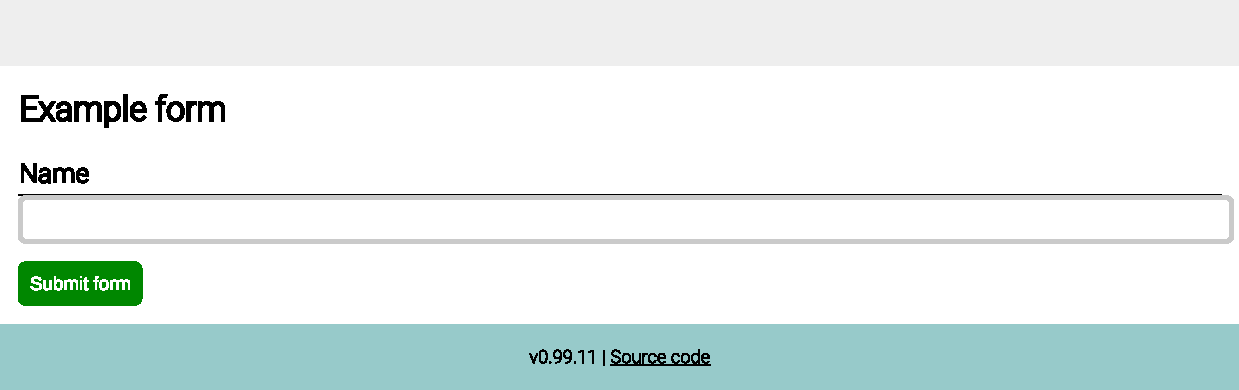
\includegraphics[width=1.0\textwidth]{figures/sg-web-form-example.pdf}
    \end{center}
    \caption{The rendering of the \t{page} procedure of our example form.}
    \label{fig:web-form-example}
  \end{figure}

\subsubsection{Implementing the \t{submit} procedure}

  The third step is to catch a form submission, which is the purpose of the
  \t{submit} procedure.  This procedure is expected to take two arguments,
  and return an SXML tree.

\begin{siderules}
\begin{verbatim}
(define (submit request-path data)
  (let* ((name (assoc-ref data 'name))
         (state (cond
                 [(or (not name)
                      (not (string-is-longer-than name 0)))
                  '(#f "Missing name.")]
                 [(string-is-longer-than name 64)
                  '(#f "Name may not be longer than 64 characters.")]
                 [else
                  '(#t)])))
    (if (car state)
        (page-empty-template "Thank you" request-path
         `((h2 "Thank you, " ,name "!")))
        (page request-path #f (cadr state)))))
\end{verbatim}
\end{siderules}

  After submitting the form, it may render in the web browser as displayed
  in figure \ref{fig:web-form-submit}.

  \begin{figure}[H]
    \begin{center}
      
\includegraphics[width=1.0\textwidth]{figures/sg-web-form-example-submit.pdf}
    \end{center}
    \caption{The rendering of the \t{submit} procedure of our example form.}
    \label{fig:web-form-submit}
  \end{figure}


\subsubsection{Implementing the \t{api} procedure}

  The final step involves implementing the optional \t{api} procedure
  that takes seven arguments:
  \begin{itemize}
  \item \t{request-path}:   The relative path of the form;
  \item \t{arguments}:      An alist of parameters passed by the URI.
  \item \t{input-port}:     The port to read data from;
  \item \t{output-port}:    The port to write data to;
  \item \t{accept-type}:    The value of the requests's \t{Accept} header;
  \item \t{content-type}:   The value of the requests's \t{Content-Type} header;
  \item \t{content-length}: The number of bytes that can be read from
    \t{input-port}.
  \end{itemize}

  This procedure is primarily designed to provide autocompletion options
  for form fields.

\begin{siderules}
\begin{verbatim}
(define (api request-path arguments input-port output-port
             accept-type content-type content-length)
  ...)
\end{verbatim}
\end{siderules}

\pagebreak{}
\section{Reports}
\label{sec:reports}

  Reports are displayed in the ``report'' section of a project.  To implement
  a report module, the following variables and procedures need to be implemented:
  \begin{itemize}
  \item \t{title}: The title for the subheading in the ``report'' page.
  \item \t{project}: The hash of the project to display the report module.
  \item \t{report-overview}: A procedure that returns an SXML tree that
    provides the content under the subheading of the report module.
  \item \t{report-pdf}: A procedure that writes a PDF stream to a given port
    that provides an archiveable record for users to download.
  \end{itemize}

\subsection{Example of a report module}

  Report modules must be placed under the \t{www reports} module prefix.

\subsubsection{The Scheme module}
\label{sec:scheme-module}

  The first part involves defining a Scheme modules with one procedure and
  two variables.

\begin{siderules}
\begin{verbatim}
(define-module (www reports example)
  #:export (title project report-overview))
\end{verbatim}
\end{siderules}

\subsubsection{Implementing \t{title} and \t{project}}

  Setting \t{title} and \t{project} involves defining two variables.

\begin{siderules}
\begin{verbatim}
(define title   "Example report")
(define project "e434cfe3752025c6fdbedbccc3f25265198da4358b0e23c77897bf7f5844ba5c")
\end{verbatim}
\end{siderules}

  Upon entering the \emph{Report} page, \t{sg-web} displays only the report
  modules that are configured for the current project.  Therefore it is
  important to ensure the value set in \t{project} matches the
  \emph{project hash} of the project intended to extend.

\subsubsection{Implementing the \t{report-overview} procedure}

  The \t{report-overview} procedure takes no argments and is expected to
  return an SXML tree that renders HTML.  The following implementation of
  the \t{report-overview} procedure renders a table.

\begin{siderules}
\begin{verbatim}
(define (report-overview)
  `(table (@ (class "item-table"))
     (tr (th "Identifier")
         (th "Description"))
     (tr (td "foo")
         (td "bar"))))
\end{verbatim}
\end{siderules}

\subsubsection{Implementing the \t{report-pdf} procedure}

  The \t{report-pdf} procedure takes a binary output port and a string as
  arguments, and is expected to write HTTP/1.1 chunked encoded output to
  the output port.  The following implementation of the \t{report-pdf}
  procedure produces a PDF report using the module \t{(www reports)}
  and writes it with the proper encoding to the output port:

\begin{siderules}
\begin{verbatim}
(define (report-pdf port identifier)
  (let ((pdf (pdf-report)))
    (pdf-report-set-title!          pdf "Example")
    (pdf-report-render-text-field!  pdf "Identifier" identifier 1)
    (pdf-report-write-to-port! port pdf #t)
    (pdf-report-close               pdf)))
\end{verbatim}
\end{siderules}

